\newcommand{\deadline}{16.06.2023}

\documentclass[11pt]{article}

\usepackage[exercise,exp]{custom_2.0}
\usepackage{amsmath}
\begin{document}

\section{Elektrische Leitfähigkeit eines Halbleiters}
\begin{adjustwidth}{20pt}{}
    Liest man den Plot so, als ob die Achsen linear wären und 
    von null in ganzen Zahlen hochzählen würden, dann ist die Funktionsverschrift
    ungefähr:
\end{adjustwidth}
\begin{align*}
    y &= 5.5 -\frac{5.5}{3.5}x  = 5.5 -\frac{11}{7}x 
\end{align*}
\begin{adjustwidth}{20pt}{}
    Aus den linear abgelesen Achsen lassen sich die Werte der 
    realen Achsen wie folgt berechnen: 
\end{adjustwidth}
\begin{align*}
    \sigma &= 10^{y-2} \implies y =\log_{10}(\sigma)\\
    \frac{1}{T} &= (0.8 + x)\cdot 10^{-3} \implies x = \frac {10^3}{T} - 0.8
\end{align*}
\begin{adjustwidth}{20pt}{}
    Setzt man dies in die gefundene Funktionsgleichung ein, folgt:
\end{adjustwidth}
\begin{align*}
    \log_{10}(\sigma)+1 &= 5.5 -\frac{11}{7}\hug{\frac {10^3}{T} - 0.8}\\
    \sigma &= 10^{\frac{403}{70} -\frac{11}{7}\frac {10^3}{T}} \\
    &\approx c_1 \cdot e^{-\frac{c_2}{T}} \with \begin{cases}
        c_1 = 5.72\cdot 10^{5}\ufrac{1}{\Omega m} \\
        c_2 = 3.62\cdot 10^{3}\u K\\
    \end{cases}\\
    &= c_1 \cdot e^{-\frac{c_2}{\tilde T + 273.15° \mathrm C}}\with c_2 = 3.62\cdot 10^{3}\u C
\end{align*}
\begin{align*}
    I &= \frac{U}{R}\\
    &= U \hug{\frac{L}{\sigma F}}^{-1}\\
    &= \frac{c_1 F U}{L} e^{-\frac{a_2}{\tilde T + 273.13\celsius}}\\
    &= \frac{5.72\cdot 10^{5}\ufrac{1}{\Omega m} \cdot 1\u{mm}^2\cdot 4 \u V}{3\u{cm}}e^{-\frac{c_2}{\tilde T + 273.13\celsius}}\\
    &\approx c_1 e^{-\frac{c_2}{\tilde T + 273.13\celsius}} \with c_1 = 76.3\u A\\
    \tilde T &= \frac{c_2}{\ln\hug{\frac{c_1}{I}}} - 273.15\celsius\\ 
    \tilde T(0.25\u A) &\approx \frac{3.62\cdot 10^{3}\u C}{\ln\hug{\frac{76.3\u A}{0.25\u A}}} -273.15\celsius\\ 
    &\approx 360\celsius
\end{align*}

\section{Zyklotronfrequenz}
\subsection{}
\begin{align*}
    F_Z &= F_L\\
    m \frac{v^2}{r} &= q v B\\
    m \frac{Uf}{r} &= q B\\
    m \frac{2\pi r}{rT} &= q B\\
    T &= \frac{2\pi m}{q B}\\
    &\approx \frac{2\pi \cdot \massproton}{\chargeproton \cdot 1.1\u T}\\
    &\approx 59.5\u{ns}
\end{align*}

\subsection{}
\begin{align*}
    F_Z &= F_L\\
    m \frac{v^2}{r} &= q v B\\
    v &= \frac{q r B}{m}\\
    &\approx \frac{\chargeproton \cdot 32 \u{cm}\cdot 1.1 \u T}{\massproton}\\
    &\approx 3.38 \cdot 10^{7}\ufrac ms \approx 0.113 \u c
\end{align*}
\begin{adjustwidth}{20pt}{}
    Obwohl das Teilchen mit einem nicht vernachlässigbaren Anteil der Lichtgeschwindigkeit fliegt,
    ist der dazugehörige Gammafaktor nur $\gamma \approx 1.0064$, sodass 
    der relative Fehler bei der Galileischen Rechnung kleiner als $1\%$ ist; Es handelt sich somit 
    immer noch um eine sehr gute Näherung.  
\end{adjustwidth}
\subsection{}
\begin{align*}
    f &= \frac 1 T\\
    &=  \frac{q B}{\pi m} \notethat \text{siehe (a)}\\
    &\approx \frac{\chargeproton \cdot 1.1\u T}{2\pi \cdot \massproton}\\
    &\approx 1.68\cdot 10^7 \ufrac 1s
\end{align*}
\begin{adjustwidth}{20pt}{}
    Die Zyklotronfrequenz ist offensichtlich nicht von $r$ abhängig.
\end{adjustwidth}

\section{Thermospannungen}
\subsection{}
\begin{adjustwidth}{20pt}{}
    Der Aufbau wird als Thermoelement bezeichnet und funktioniert
    aufgrund des Seebeck-Effektes.
\end{adjustwidth}

\subsection{}
\begin{align*}
    U_M &= (k_{\mathrm{Konst},\mathrm{Pt}} - k_{\mathrm{Ni-Cr},\mathrm{Pt}})(T_1-T_2)\\
    &\approx \hug{-3.2 \ufrac{mV}{100K} - 2.2 \ufrac{mV}{100K}} (200\celsius - 40\celsius\ \, )\\
    &\approx -8.64 \, \u{mV} 
\end{align*}

\section{Galvanische Vernickelung}
\subsection{}
\begin{align*}
    I_{max} &= j_{max}A = j_{max}(2\pi r^2 + 2\pi r l) = 2 \pi r j_{max}(r + l)\\
    &\approx 2\pi \cdot 30\ufrac{A}{m^2} \cdot 5\u{cm}(5\u{cm} + 75\u{cm})\\
    &\approx 7.54\u{A}
\end{align*}

\subsection{}
\begin{align*}
    {\mathrm A_c} &= m_{Ni}n = m_{Ni} \frac{1\u C}{2 \abs{q} n_A}\\
    &\approx 58.69\u u \frac{1 \u C}{2 \cdot \chargeproton \cdot \avogadro}\\
    &\approx 304 \u {n g}\\
\end{align*}

\subsection{}
\begin{align*}
    V_{neu} &= \pi (r+\delta)^2 (l+2\cdot \delta) - \pi r^2 l \\
    &= \pi \delta \hug{2 r l + \delta (l+4 r) + \delta^2}\\
    Q_{ges} &= \frac{m_{neu}}{A_c} \\
    &= \frac{p_{Ni}V_{neu}}{A_c}
\end{align*}
\begin{align*}
    t_{ges} &= \frac{Q_{ges}}{I_{max}}\\
    &= \frac{p_{Ni}\pi \delta \hug{2 r l + \delta (l+4 r) + \delta^2}}{\mathrm A_c I_{max}}\\
    &\approx \frac{\pi\cdot 8.9\ufrac{g}{cm^3} \cdot 0.15\u{mm} \hug{2 \cdot 5\u{cm} \cdot 75\u{cm} + 0.15\u{mm} (75\u{cm}+4 \cdot 5\u{cm}) 
    + 0.15^2\u{mm}^2}}{304 \u {ng}\cdot  7.54\u{A}}\\
    &\approx 38.1\u h
\end{align*}


\section{Massenspektrometer}
\subsection{}
\begin{adjustwidth}{20pt}{}
    Die Flugbahn der Na$^+$-Ionen ist ein Halbkreis, da die Lorenzkraft 
    immer orthogonal zum Geschwindigkeitsvektor ist, und somit
    als Zentripetalkraft fungiert.
\end{adjustwidth}
\begin{align*}
    E_{kin} &= E_{el}\\
    \frac{m v^2}{2} &= n q U\\
    v &= \sqrt{\frac{2 n q U}{m}}\\
    \\
    F_Z &= F_L\\
    m \frac{v^2}{r} &= q v B\\
    m \sqrt{\frac{2 n q U}{m}} &= q r B\\
    m  &= \frac{q r^2 B^2}{2 n U}\\
    &\overset{(1)}{\approx} \frac{\chargeproton \cdot \frac{1.38^2 \u m^2}{2}\cdot 1.0^2 \u T^2}{2\cdot 1\cdot 100 \u V}\\
    &\approx 7.63\cdot 10^{-22} \u{kg}
\end{align*}
\begin{adjustwidth}{20pt}{}
    $(1):$ Es wurde angenommen, dass die Natriumionen nur einfach positiv geladen sind.
\end{adjustwidth}

\subsection{}
\begin{adjustwidth}{20pt}{}
    Man könnnte einen Geschwindigkeitsfilter mit Hilfe eines E/- und eines B-Feldes
    konstruieren, indem man in dem Aufbau aus (a) das B-Feld mit einem 
    homogenen E-Feld überlagert, welches die Ladungsträger in die entgegengesetzte Richtung 
    beschleunigt, d.h. in der Skizze wäre rechts der positive Pol.
    So würden nur die Partikel geradeaus fliegen, für die die Kraft der E-Feldes 
    perfekt durch das B-Feld negiert wird. Da beide Kräfte proportialional
    zur Ladung sind, kürzt sich diese weg, und es bleibt ein Ausdruck 
    der nur von E-/B-Feld abhängt. Da 
    E-/ und B-Feldstärke als bekannt und einstellbar angenommen werden,
    lässt sich somit, durch geschicktes Einstellen der Felder, nach der Geschwindigkeit 
    von Ladungsträgern selektieren. 
\end{adjustwidth}
\begin{align*}
    F_L &= F_{el}\\
    q v B &= q E\\
    v &= \frac{E}{B}
\end{align*}
\begin{adjustwidth}{20pt}{}
    Nachteile dieses Aufbaus zur Geschwindigkeitsbestimmung sind, dass die Teilchen 
    Ladungsträger sein müssen, und dass bei kleinen Geschwindigkeiten 
    die Erdbeschleunigung das Instrument nutzlos machen würde.
\end{adjustwidth}

\subsection{}
\begin{adjustwidth}{20pt}{}
    Sei der Eintrittsspalt der Ursprung des Koordinatensystems, die X-Achse der Schirm.
    Dann ist die Flugbahn eines positiven Ladungsträgers im homogenen B-Feld
    ein Kreis mit Radius $r$, dessen Rand durch den Ursprung geht und dessen Tangente
    in diesem Punkt mit der Y-Achse den Winkel $\alpha$ einschließt.
\end{adjustwidth}

\begin{figure}[h]
    \centering
    \hspace{\fill}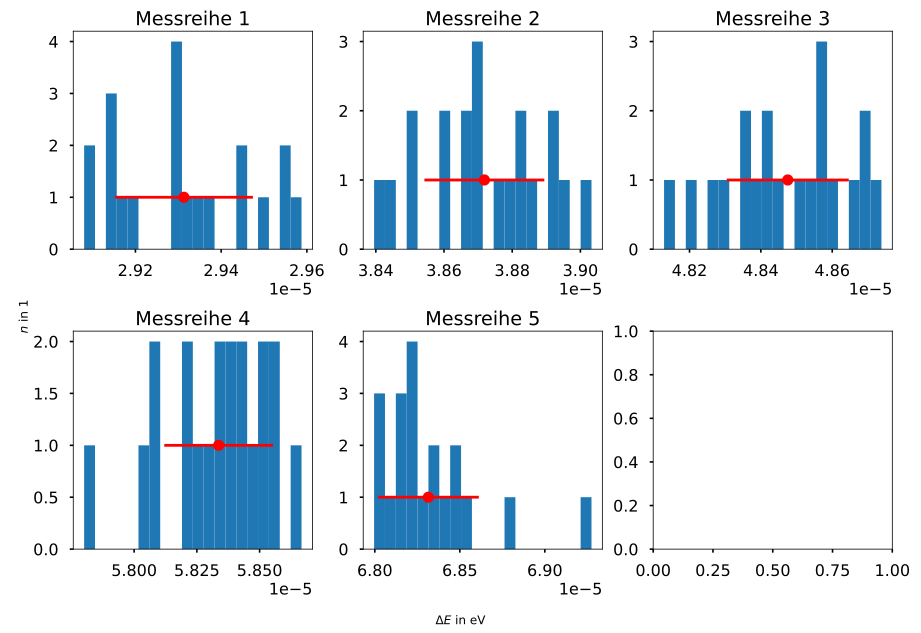
\includegraphics[width=0.4\textwidth]{1}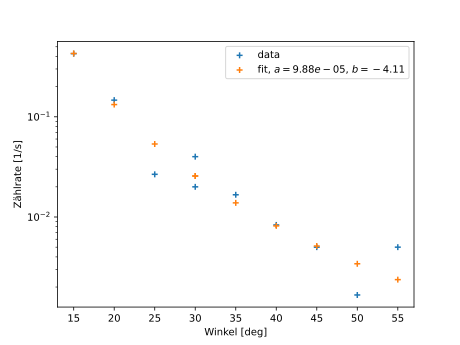
\includegraphics[width=0.4\textwidth]{2}\hspace*{\fill}
    \caption{Flugbahnen mit verschiedenen $\alpha$}
\end{figure}

\begin{adjustwidth}{20pt}{}
    In Polarkoordinaten lässt sich somit die folgende Gleichung für die Flugbahn aufstellen: 
\end{adjustwidth}
\begin{align*}
    r(\phi) &= R\cdot \cos(\phi + \alpha)
\end{align*}
\begin{adjustwidth}{20pt}{}
    Für die Kollision mit dem Schirm muss $\phi=0$ gelten:
\end{adjustwidth}
\begin{align*}
    r_0 &= R\cdot \cos(\alpha)\\
    &\approx R \hug{1-\frac{\alpha^2}{2}} \for \abs{\alpha} \ll 1\\
    \Delta r_0 &= r_0(0^\circ) - r_0(\alpha)\\
    &= R(1-\cos(\alpha)) \\
    &\approx \frac{\alpha^2 R}{2 } \for \abs{\alpha} \ll 1\\
    \Delta r_0 (3^\circ)&\approx \frac{\alpha^2 R}{2 }  
    = \frac{\alpha^2 x}{4 }\\
    &\approx \hug{\frac{3\cdot 2\pi}{360}}^2 \frac{1.38\u{cm}}{4}\\
    &\approx 9.46\cdot 10^{-6}\u m
\end{align*}

\end{document}